\item \begin{theorem}{(429)} Pipeline不會對單一工作的latency有幫助,但會提升整體工作的throughput。
\end{theorem}

\item \begin{theorem}{(441)} 原始pipeline設計:\begin{itemize}
        \item \code{beq}在$MEM$決定是否要跳。
        \item \code{RegDst}在$EX$。
    \end{itemize}
    \begin{figure}[H]
        \centering
        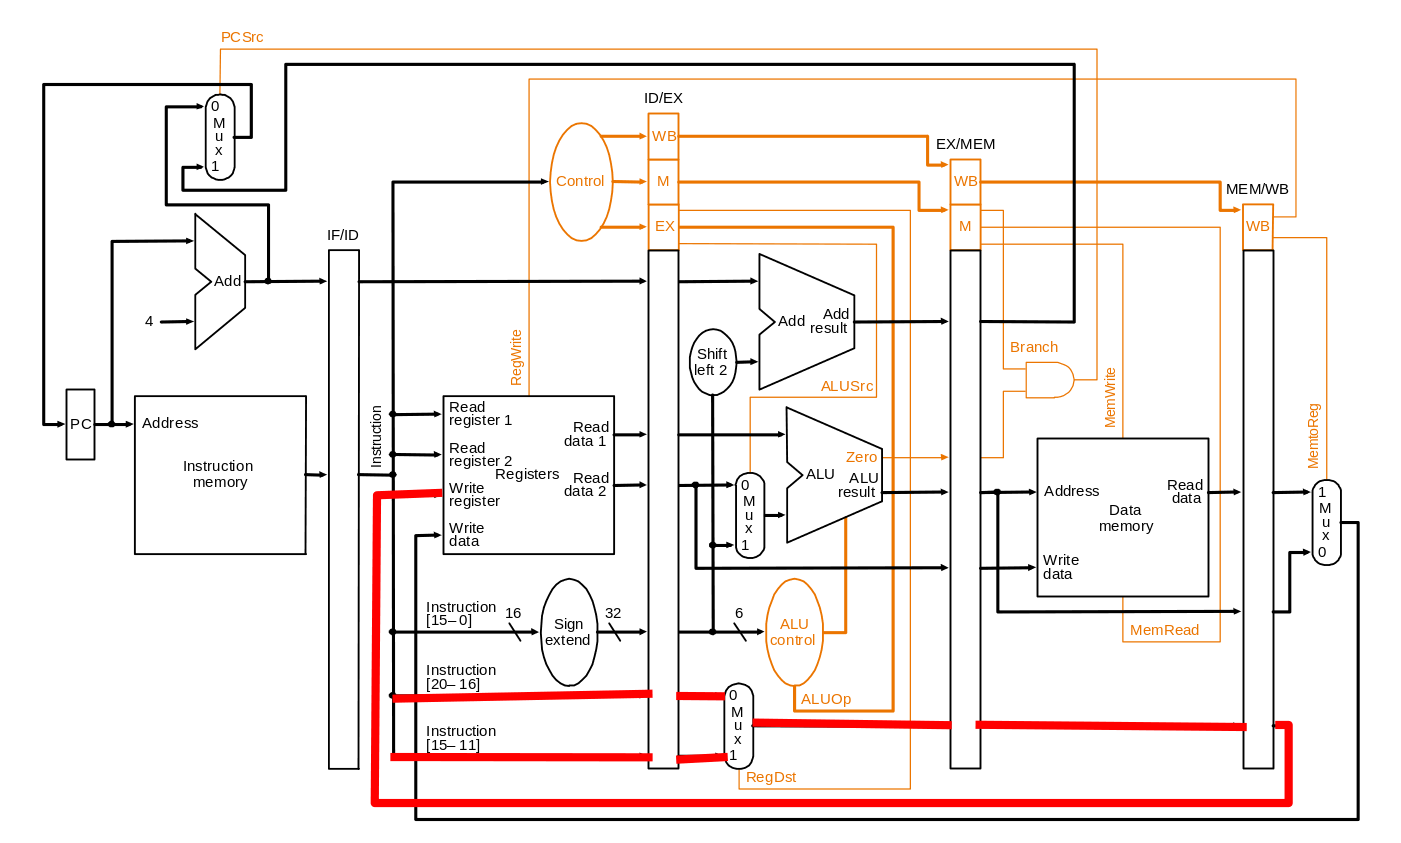
\includegraphics[scale=0.3]{img/pipeline-org.png}
        \caption{Original pipeline.}
        \label{img:pipeline-org}
    \end{figure}
    \begin{table}[H]
        \centering
        \begin{tabular}{|c|c|c|c|c|c|}
            \hline
            Stage & $IF$ & $ID$ & $EX$ & $MEM$ & $WB$ \\
            \Xhline{2\arrayrulewidth}
            Signal & $\texttimes$ & $\texttimes$ & \makecell{RegDst\\ALUSrc\\ALUOp} & \makecell{MemRead\\MemWrite\\branch} & \makecell{RegWrite\\MemtoReg} \\
            \hline
        \end{tabular}
    \end{table}
\end{theorem}

\item \begin{theorem}{()} NOP無法解決structual hazard,因為NOP本質上也是指令。
\end{theorem}

\item \begin{theorem}{(450, 455, 457, 458)} Data hazards:\begin{itemize}
        \item Insert NOP:\code{slt $0, $0, 0},浪費$2$ CC。
        \item Forwarding:Combinational units,放在$EX$因為$ALU$。
        \begin{lstlisting}[caption={EX hazard.}, captionpos=b, mathescape=true, language={[x86masm]Assembler}]
            if (EX/MEM.RegWrite $\land$ (EX/MEM.Rd $\neq 0$) $\land$ (EX/MEM.Rd $=$ ID/EX.Rs/Rt))
                ForwardA/B = $10$
        \end{lstlisting}
        \begin{lstlisting}[caption={MEM hazard.}, captionpos=b, mathescape=true, language={[x86masm]Assembler}]
            if (MEM/WB.RegWrite $\land$ (MEM/WB.Rd $\neq 0$) $\land$ ($\lnot$ EX_hazard) $\land$ (MEM/WB.Rd $=$ ID/EX.Rs/Rt))
                ForwardA/B = $01$
        \end{lstlisting}
        \begin{figure}[H]
            \centering
            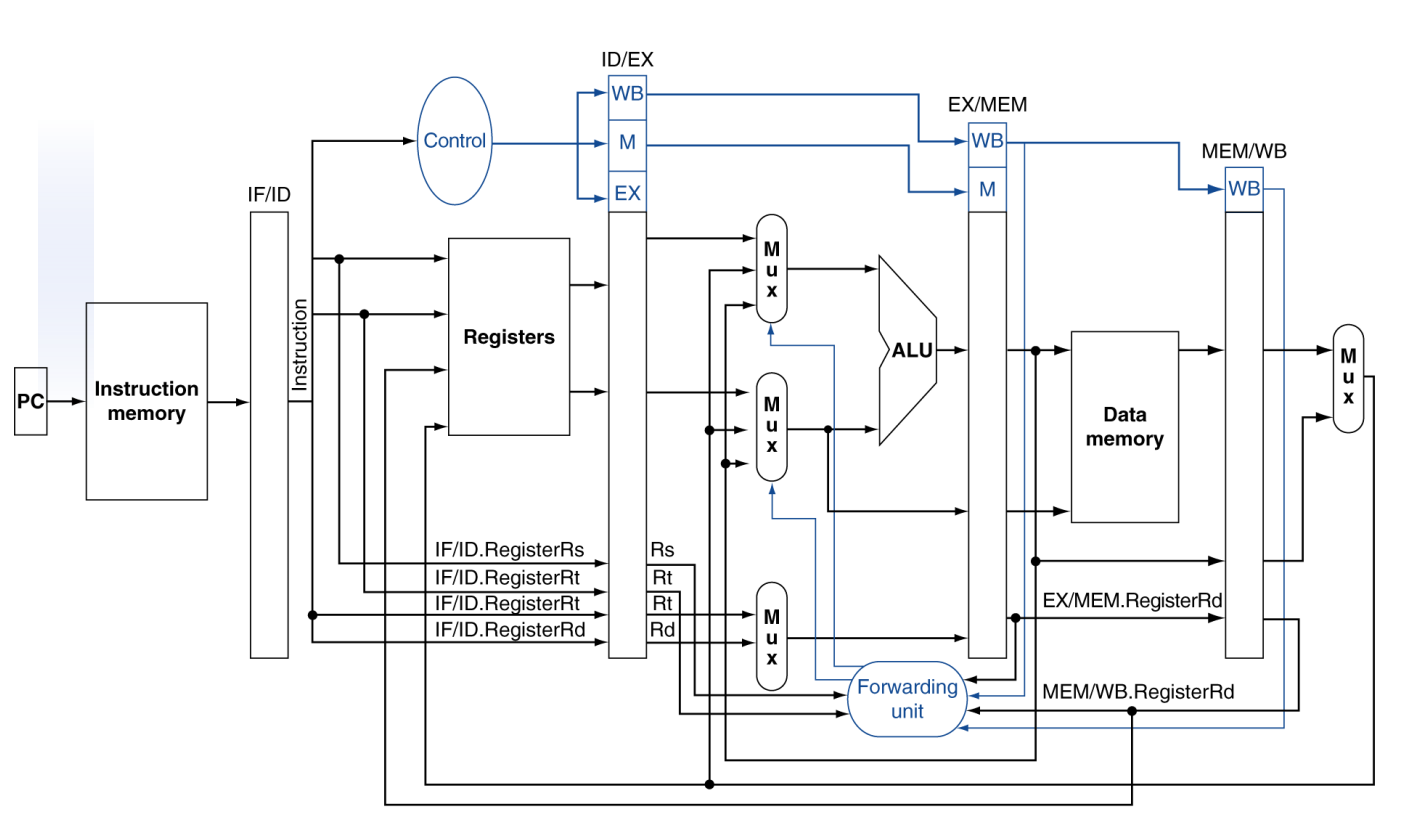
\includegraphics[scale=0.3]{img/pipeline-forward.png}
            \caption{Pipeline with forwarding.}
            \label{img:pipeline-forward}
        \end{figure}
        \item Stall:\code{}
        \begin{lstlisting}[caption={Stall.}, captionpos=b, mathescape=true, language={[x86masm]Assembler}]
            if (ID/EX.MemRead $\land$ (ID/EX.Rt $=$ IF/ID.Rs/Rt))
                IF/ID.Write := $0$
                PC.Write := $0$
        \end{lstlisting}
        \begin{figure}[H]
            \centering
            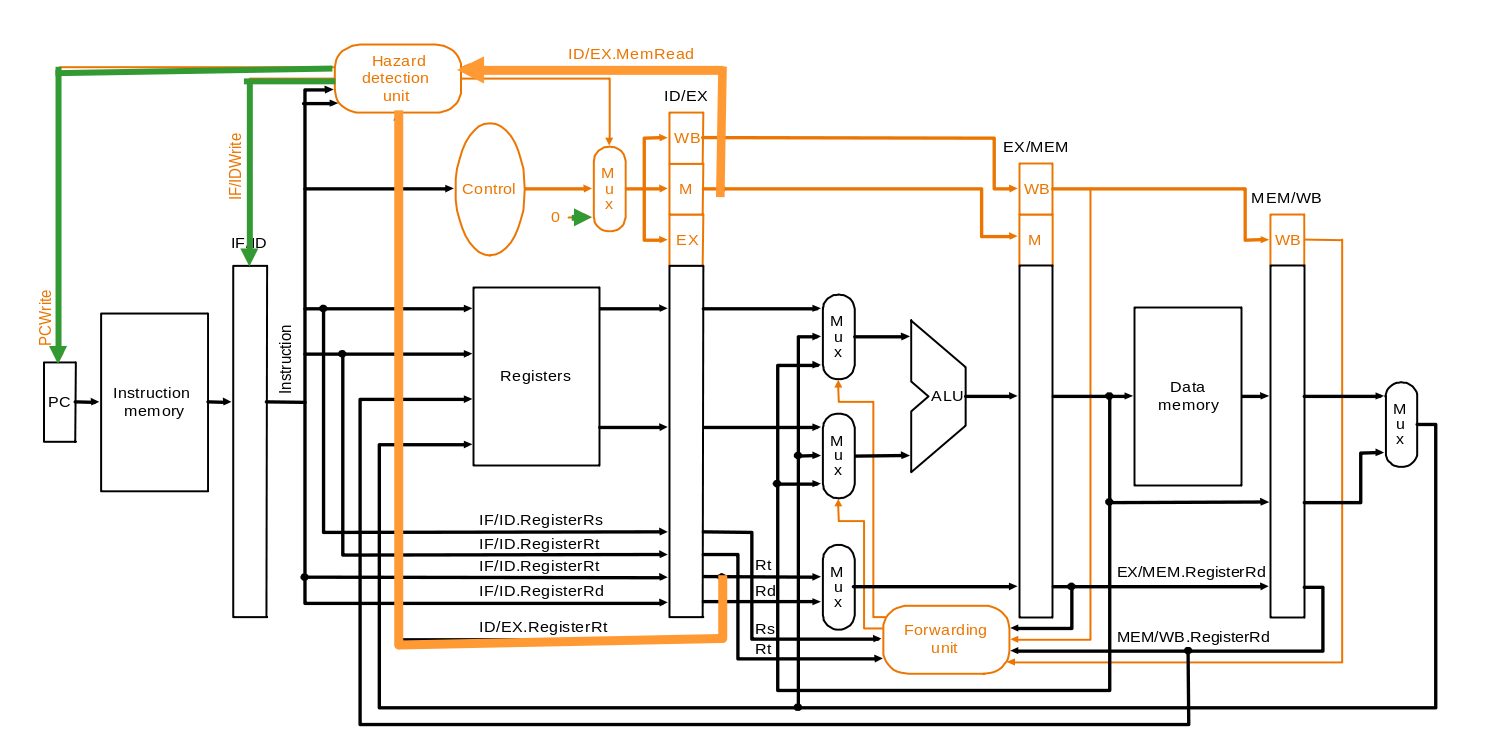
\includegraphics[scale=0.3]{img/pipeline-hazard.png}
            \caption{Pipeline with hazard detection and forwarding units.}
            \label{img:pipeline-hazard}
        \end{figure}
    \end{itemize}
\end{theorem}

\item \begin{theorem}{(473)} RAW: True data dependency.
\end{theorem}

\item \begin{theorem}{(478, 487, 494, 559)} Control hazards:\begin{itemize}
        \item 若分支指令與\textbf{前一個ALU指令}或\textbf{前面第二個}\code{lw}有data dependency,必須stall $1$ CC。
        \item 若分支指令與\textbf{前一個}\code{lw}有data dependency,必須stall $2$ CC。
        \item 分支指令通過$XOR$再$NOR$比較是否相同。
        \begin{figure}[H]
            \centering
            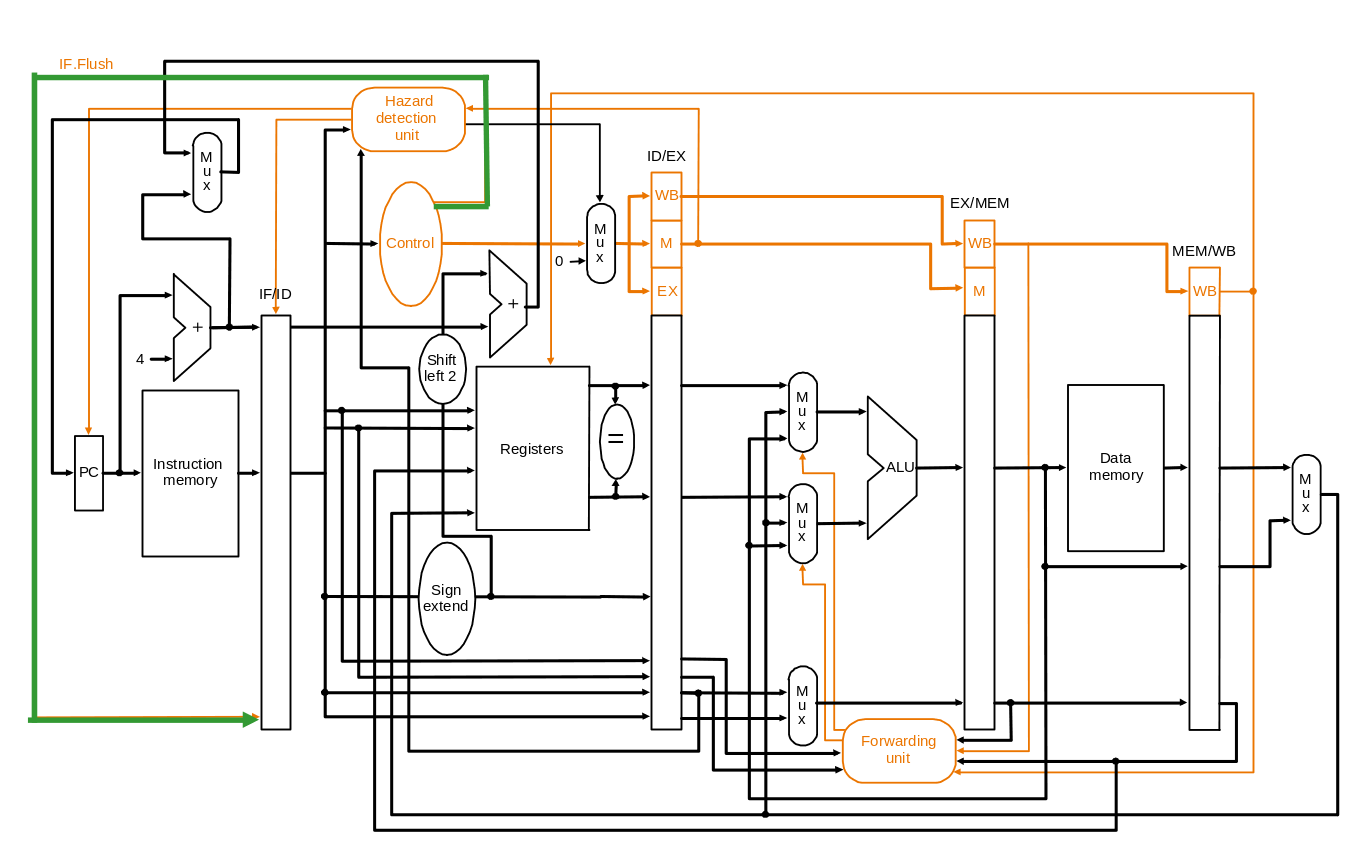
\includegraphics[scale=0.3]{img/pipeline-flush.png}
            \caption{Pipeline with hazard detection, forwarding units and flush.}
            \label{img:pipeline-flush}
        \end{figure}
        \item Branch Target Buffer (BTB) check the branch in $IF$.
        \item Delayed branch:\begin{itemize}
            \item NOT suitable for deep pipeline.
            \item From before:最佳方法,不管跳或不跳皆提升。
            \item From target:用於branch發生機率高。
            \item From fall through:用於branch發生機率低。
            \begin{figure}[H]
                \centering
                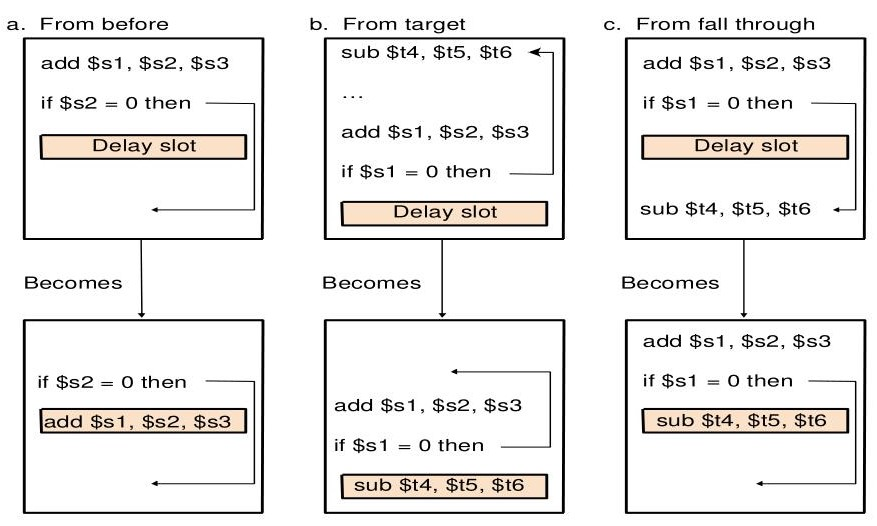
\includegraphics[scale=0.6]{img/delayed-branch.jpg}
                \caption{Example of delayed branch.}
                \label{img:delayed-branch}
            \end{figure}
        \end{itemize}
    \end{itemize}
\end{theorem}

\item \begin{theorem}{(498)} Advanced pipeline:\begin{itemize}
        \item Instruction-Level Parallelism (ILP):\begin{itemize}
            \item Increase pipeline depth:superpipeline,但hazard也上升。
            \item Multiple issue:大量複製pipeline單元,讓每個stage都可以執行多個指令。\begin{itemize}
                \item 可分為static和dynamic,前者在編譯時決策,MIPS64採用,後者在執行時決策,又稱super scaler。
                \item Static:軟體實現,Code scheduling, loop unrolling, Very Long Instruction Word (VLIW).
                \item Dynamic:硬體實現,pipeline被分為in-order issue units,out-of-order execute units和in-order commit units。
            \end{itemize}
        \end{itemize}
        \item Speculation:猜測指令的性質,以便執行其他相關指令。軟硬體共同實現。
    \end{itemize}
\end{theorem}

\item \begin{theorem}{(515)} Exception:\begin{itemize}
        \item Exception:內部;Interrupt:外部。
        \item Exception Program Counter (EPC):存放引發exception指令地址;Status/Cause register:存放exception原因。
        \item Imprecise interrupt:不知道發生的stage,只能kill program。
    \end{itemize}
\end{theorem}
